\documentclass{article}

\usepackage{fancyhdr}
\usepackage{extramarks}
\usepackage{amsmath}
\usepackage{amsthm}
\usepackage{amsfonts}
\usepackage{tikz}
\usepackage[plain]{algorithm}
\usepackage{algpseudocode}
\usepackage{tikz,pgfplots,multicol}
\usepackage[font=small,labelformat=empty]{caption}
\usetikzlibrary{automata,positioning}

%
% Basic Document Settings
%

\topmargin=-0.45in
\evensidemargin=0in
\oddsidemargin=0in
\textwidth=6.5in
\textheight=9.0in
\headsep=0.25in

\linespread{1.1}

\pagestyle{fancy}
\lhead{\hmwkAuthorName}
\chead{\hmwkClass\ (\hmwkClassInstructor\ \hmwkClassTime)}
\rhead{\hmwkTitle}
\lfoot{\lastxmark}
\cfoot{\thepage}

\renewcommand\headrulewidth{0.4pt}
\renewcommand\footrulewidth{0.4pt}

\setlength\parindent{0pt}

\setcounter{secnumdepth}{0}
\newcounter{partCounter}
\newcounter{homeworkProblemCounter}
\setcounter{homeworkProblemCounter}{1}
\nobreak\extramarks{Problem \arabic{homeworkProblemCounter}}{}\nobreak{}

%
% Homework Problem Environment
%
% This environment takes an optional argument. When given, it will adjust the
% problem counter. This is useful for when the problems given for your
% assignment aren't sequential. See the last 3 problems of this template for an
% example.
%
\newenvironment{homeworkProblem}[1][-1]{
    \ifnum#1>0
        \setcounter{homeworkProblemCounter}{#1}
    \fi
    \section{Problem \arabic{homeworkProblemCounter}}
    \setcounter{partCounter}{1}
    \enterProblemHeader{homeworkProblemCounter}
}{
    \exitProblemHeader{homeworkProblemCounter}
}

%
% Homework Details
%   - Title
%   - Due date
%   - Class
%   - Section/Time
%   - Instructor
%   - Author
%

\newcommand{\hmwkTitle}{HW \#5}
\newcommand{\hmwkDueDate}{February 16, 2017}
\newcommand{\hmwkClass}{MATH 1300}
\newcommand{\hmwkClassTime}{Section 005}
\newcommand{\hmwkClassInstructor}{Professor Braden Balentine}
\newcommand{\hmwkAuthorName}{\textbf{John Keller}}

%
% Title Page
%

\title{
    \vspace{2in}
    \textmd{\textbf{\hmwkClass:\ \hmwkTitle}}\\
    \normalsize\vspace{0.1in}\small{Due\ on\ \hmwkDueDate\ at 10:00am}\\
    \vspace{0.1in}\large{\textit{\hmwkClassInstructor\ \hmwkClassTime}}
    \vspace{3in}
}

\author{\hmwkAuthorName}
\date{}

\renewcommand{\part}[1]{\textbf{\large Part \Alph{partCounter}}\stepcounter{partCounter}\\}

%
% Various Helper Commands
%

% Useful for algorithms
\newcommand{\alg}[1]{\textsc{\bfseries \footnotesize #1}}

% For derivatives
\newcommand{\deriv}[1]{\frac{\mathrm{d}}{\mathrm{d}x} (#1)}

% For partial derivatives
\newcommand{\pderiv}[2]{\frac{\partial}{\partial #1} (#2)}

% Integral dx
\newcommand{\dx}{\mathrm{d}x}

% Alias for the Solution section header
\newcommand{\solution}{\textbf{\large Solution}}

% Probability commands: Expectation, Variance, Covariance, Bias
\newcommand{\E}{\mathrm{E}}
\newcommand{\Var}{\mathrm{Var}}
\newcommand{\Cov}{\mathrm{Cov}}
\newcommand{\Bias}{\mathrm{Bias}}

\begin{document}

\maketitle

\pagebreak

\section{Graphical Problems}

\begin{enumerate}
\setcounter{enumi}{0}
	\item Find the coordinates of A, B, and C.
		\begin{center}
		\pgfplotsset{width=0.6\linewidth,height=8cm,xtick={4.8,5,5.3},ytick={12}}
			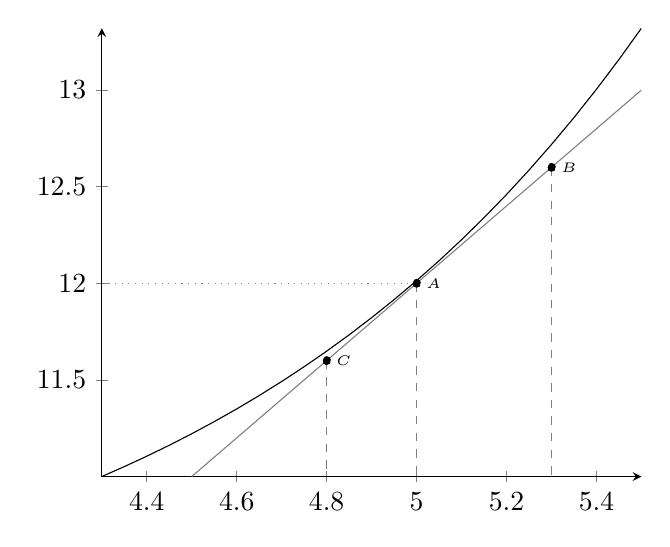
\begin{tikzpicture}
			\begin{axis}[axis lines=middle]
				\addplot[domain=4.3:5,gray,dotted] {12};
				\addplot[domain=4.3:5.5] {exp(x-4.3)+10};
				\addplot[domain=4.5:5.5,gray] {2*x+2} node[right,pos=1] {$y=2x+2$};
				\addplot[domain=0:6,gray,dashed] coordinates {(4.8,11.6)(4.8,11)};
				\addplot[domain=0:6,gray,dashed] coordinates {(5,12)(5,11)};
				\addplot[domain=0:6,gray,dashed] coordinates {(5.3,12.6)(5.3,11)};
				\addplot+[only marks,mark=*,mark options={fill=black,scale=0.7},text mark as node=false,black] coordinates {(5.3,12.6)} node[right,pos=1] {\tiny{$B$}};
				\addplot+[only marks,mark=*,mark options={fill=black,scale=0.7},text mark as node=false,black] coordinates {(5,12)} node[right,pos=1] {\tiny{$A$}};
				\addplot+[only marks,mark=*,mark options={fill=black,scale=0.7},text mark as node=false,black] coordinates {(4.8,11.6)} node[right,pos=1] {\tiny{$C$}};
			\end{axis}
		\end{tikzpicture}
		\end{center}
	$$f(5)=12 \qquad f'(5)=2$$
	\begin{itemize}
		\item Equation for tangent line: $y=2x+2$
		\item A = (5,12)
		\item B = (4.8,11.6); $\quad 2(4.8)+2=9.6+2=11.6$
		\item C = (5.3,12.6); $\quad 2(5.3)+2=10.6+2=12.6$
	\end{itemize}
	\item If possible, find each of the following values. Write "not enough information" where appropriate.
	\begin{center}
		\pgfplotsset{width=0.6\linewidth,height=6cm}
%\pgfplotsset{xmin=-3,xmax=10,ymin=-4,ymax=10,soldot/.style={color=blue,only marks,mark=*}
			\begin{tikzpicture}
			\begin{axis}[axis lines=none]
				\addplot[domain=2.5:3.5] {-exp(x-2.1)+9.45}node[bottom,pos=1] {$g(x)$};
				\addplot[domain=2.5:3.5,gray] {(-2.5)*x+14.5};
				\addplot+[only marks,mark=*,mark options={fill=black,scale=0.7},text mark as node=false,black] coordinates {(3,7)} node[right,pos=1] {$(3,7)$};
				\addplot+[only marks,mark=*,mark options={fill=black,scale=0.7},text mark as node=false,black] coordinates {(2.8,7.5)} node[right,pos=1] {$(2.8,7.5)$};
			\end{axis}
		\end{tikzpicture}
	\end{center}
	\begin{enumerate}
		\item $g(3)=7$
		\item $g(2.8)=$ Not enough information
		\item $g(7)=$ Not enough information
		\item $g^{-1}(7)=g\Big(\frac{1}{7}\Big)=$ Not enough information
		\item $g'(7)=$ Not enough information
		\item $g'(3)=-2.5$
		\item $g'(2.8)=$ Not enough information
	\end{enumerate}
\end{enumerate}

\section{Section 2.8}
\begin{enumerate}
\setcounter{enumi}{8}
	\item The president announces that the national deficit is increasing, but at a decreasing rate. Interpret this statement in terms of a function and its derivatives.\newline
	The president's statement can be described by mathematical terms by saying the derivative of the national deficit is slowly decreasing, due to the slope of the deficit lessening as time goes on.
\setcounter{enumi}{21}
	\item Sketch the graph of a function that satisfies all of the given conditions:\newline
		\begin{equation}
		\begin{split}
		f'(1)&=f'(-1)=0\\
		f'(x)<0 &\text{ if } |x| < 1\\
		f'(x)>0 &\text{ if } 1 < |x| < 2\\
		f'(x)=-1 &\text{ if } |x|>2 \\
		f''(x)<0 &\text{ if } -2 < x < 0\\
		\text{inflection point (0,1)}
		\end{equation}
		\end{split}
		
	\begin{center}
		\pgfplotsset{width=0.8\linewidth,height=10cm,xmin=-1-7,xmax=7}
%		\pgfplotsset{xmin=-10,xmax=10,ymin=-4,ymax=6,soldot/.style={color=blue,only marks,mark=*}
			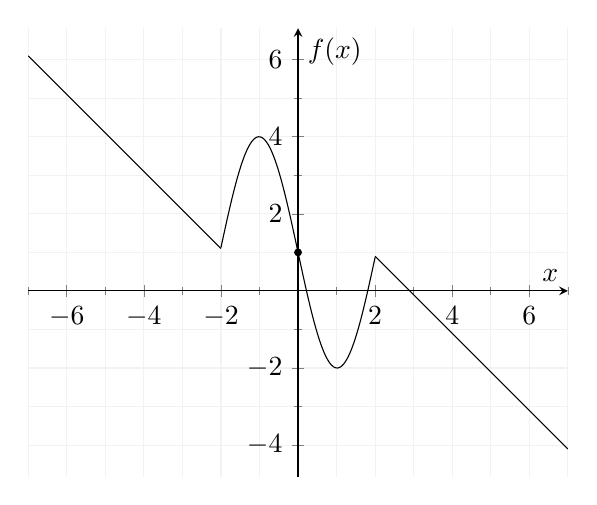
\begin{tikzpicture}
			\begin{axis}[axis lines=middle,xlabel=$x$,ylabel=$f(x)$,axis equal,grid=both,minor tick num=1,grid style={solid, gray!10}]
				\addplot[samples=100,domain=-2:2,black] {-3*sin(deg(1.55*x))+1};
				\addplot[domain=-7:-2,black] {-x-0.9};
				\addplot[domain=2:7,black] {-x+2.9};
				\addplot+[only marks,mark=*,mark options={fill=black,scale=0.6},text mark as node=false,black] coordinates {(0,1)};
				%\addplot+[only marks,mark=*,mark options={fill=black,scale=0.7},text mark as node=false,black] coordinates {(1.52,0.5)};
				%\addplot[domain=-2:0,gray,dashed] {4} node[right,pos=1] {\tiny{${f'(-1)=0}$}};
				%\addplot[domain=0:2,gray,dashed] {-2} node[right,pos=1] {\tiny{${f'(1)=0}$}};
			\end{axis}
		\end{tikzpicture}
	\end{center}
		
\setcounter{enumi}{24}
	\item Suppose $f'(x)=xe^{-x^2}$.
\def\crulefill{\leaders\hrule
  height \dimexpr\fontdimen22\textfont2+0.2pt\relax
  depth -\dimexpr\fontdimen22\textfont2-0.2pt\relax
  \hfill
}
\def\hollow{$\kern-.8pt\circ\kern-.8pt$}
\def\filled{$\kern-.8pt\bullet\kern-.8pt$}

$$
\vbox{\offinterlineskip\tabskip=0pt
  \halign{%
    \strut$#$\hfil\quad&
    \hfil\qquad$#$\qquad\hfil&
    \hfil\vrule#\hfil&
    \hfil\qquad$#$\qquad\hfil&
    \hfil\vrule#\hfil&
    \hfil\qquad$#$\qquad\hfil\cr
  f(x)&-&&+&&-\cr
  \multispan{2}\crulefill&\omit\hfil\hollow\hfil&
    \omit\crulefill&\omit\hfil\hollow\hfil&\omit\crulefill\cr
  & &\omit\hidewidth$-0.707$\hidewidth& &\omit\hidewidth$0.707$\hidewidth& \cr
}}
$$

	\begin{enumerate}
		\item On what interval is $f$ increasing? On what interval is $f$ decreasing?\newline
		\begin{minipage}[t]{0.5\linewidth}
			Increasing: $(-\infty, -0.707)\cup(0.707, \infty)$
		\end{minipage}
		\begin{minipage}[t]{0.5\linewidth}
			Decreasing: $(-0.707,0.707)$
		\end{minipage}
		\item Does $f$ have a maximum value? Minimum value?\newline
			The minimum is -0.707, and the maximum is 0.707.
	\end{enumerate}
\end{enumerate}

\section{Section 3.1}
\begin{enumerate}
\setcounter{enumi}{47}
	\item On what interval is the function $f(x)=x^3-4x^2+5x$ concave upward? $(1.5,\infty)$
		\begin{center}
		\pgfplotsset{width=0.8\linewidth,height=7cm,xmin=-2, xmax=5}
%		\pgfplotsset{xmin=-10,xmax=10,ymin=-4,ymax=6,soldot/.style={color=blue,only marks,mark=*}
			\begin{tikzpicture}
			\begin{axis}[axis lines=middle,xlabel=$x$,ylabel=$f(x)$,minor tick num=1,grid style={solid, gray!20}]
				\addplot[samples=200,domain=-2:1.5,dashed,gray] {x^3-4*x^2+5*x};
				\addplot[samples=200,domain=1.5:5] {x^3-4*x^2+5*x};
			\end{axis}
		\end{tikzpicture}
		\end{center}
\setcounter{enumi}{61}
	\item The equation $y''+y'-2y=x^2$ is called a \textbf{differential equation} because it involves an unknown function $y$ and its derivatives $y'$ and $y''$. Find constants $A$, $B$, and $C$ which that the function $y=Ax^2+Bx+C$ satisfies this equation.
	$$\begin{align}
		y''+y'-2y&=x^2\\
		-2y&=x^2-y'-y''\\
		y&=-\frac{2}{3}x^2+\frac{1}{2}y'+\frac{1}{2}y''
	\end{align}\qquad
	\boxed{A=-\frac{1}{2}\quad B=\Big(\frac{1}{2}y'+\frac{1}{2}y''\Big)\quad C=0}$$
\setcounter{enumi}{65}
	\item Suppose the curve $y=x^4+ax^3+bx^2+cx+d$ has a tangent line when $x=0$ with equation $y=2x+1$ and a tangent line when $x=1$ with equation $y=2-3x$. Find the values of $a$, $b$, $c$, and $d$.
	
	$$\begin{align}
		2 &= 4(0)^3 + 3a(0)^2 + 2b(0) + c &\qquad 1 &= 0^4 + a(0)^3 + b(0)^2 + c(0) + d \\
	 	c &= 2 &\qquad d&=1
	\end{align}$$\\
	$$\begin{align}
		-3 &= 4(1)^3 + 3a(1)^2 + 2b(1) + c &\qquad -1 &= (-1)^4 + a(-1)^3 + b(-1)^2 + c(-1) + d\\
		3a + 2b + c &= -3 &\qquad -a + b - c + d + 1 &= -1\\
		3a + 2b + 2 &= -3 &\qquad  -a + b - 2 + 1 &= -2\\
		 3a + 2b &= -5 &\qquad  -a + b - 2 + 1 &= -2 \\
		 3a&=-5-2b &\qquad -a + b &= -1\\
		 a&=-\frac{5}{3}-\frac{2}{3}b &\qquad &\\
	\end{align}$$
	Now combining the two:
	$$a=-\frac{3}{5}\qquad b=-\frac{8}{5}$$
\end{enumerate}

\end{document}